\section*{Problem 3: Surface Brightness}

Ah this is a classic, and counter intuitive derivation in any atmospheres \& radiative transfers class.  (Which I have taken). The answer is that there is a $1/r^2$ factor from the flux, there is also a factor in angular size  which precisely cancel. 

I'm gonna do the full derivation + a diagram because I enjoy this problem. 

the specific surface brightness aka specific intensity is the energy emitted per unit time per unit area per unit frequency per unit solid angle:

\begin{equation}
    I_\nu = \frac{dE}{(\cos\theta dA)dtd\nu d\Omega}
\end{equation}

\begin{figure}
    \centering
    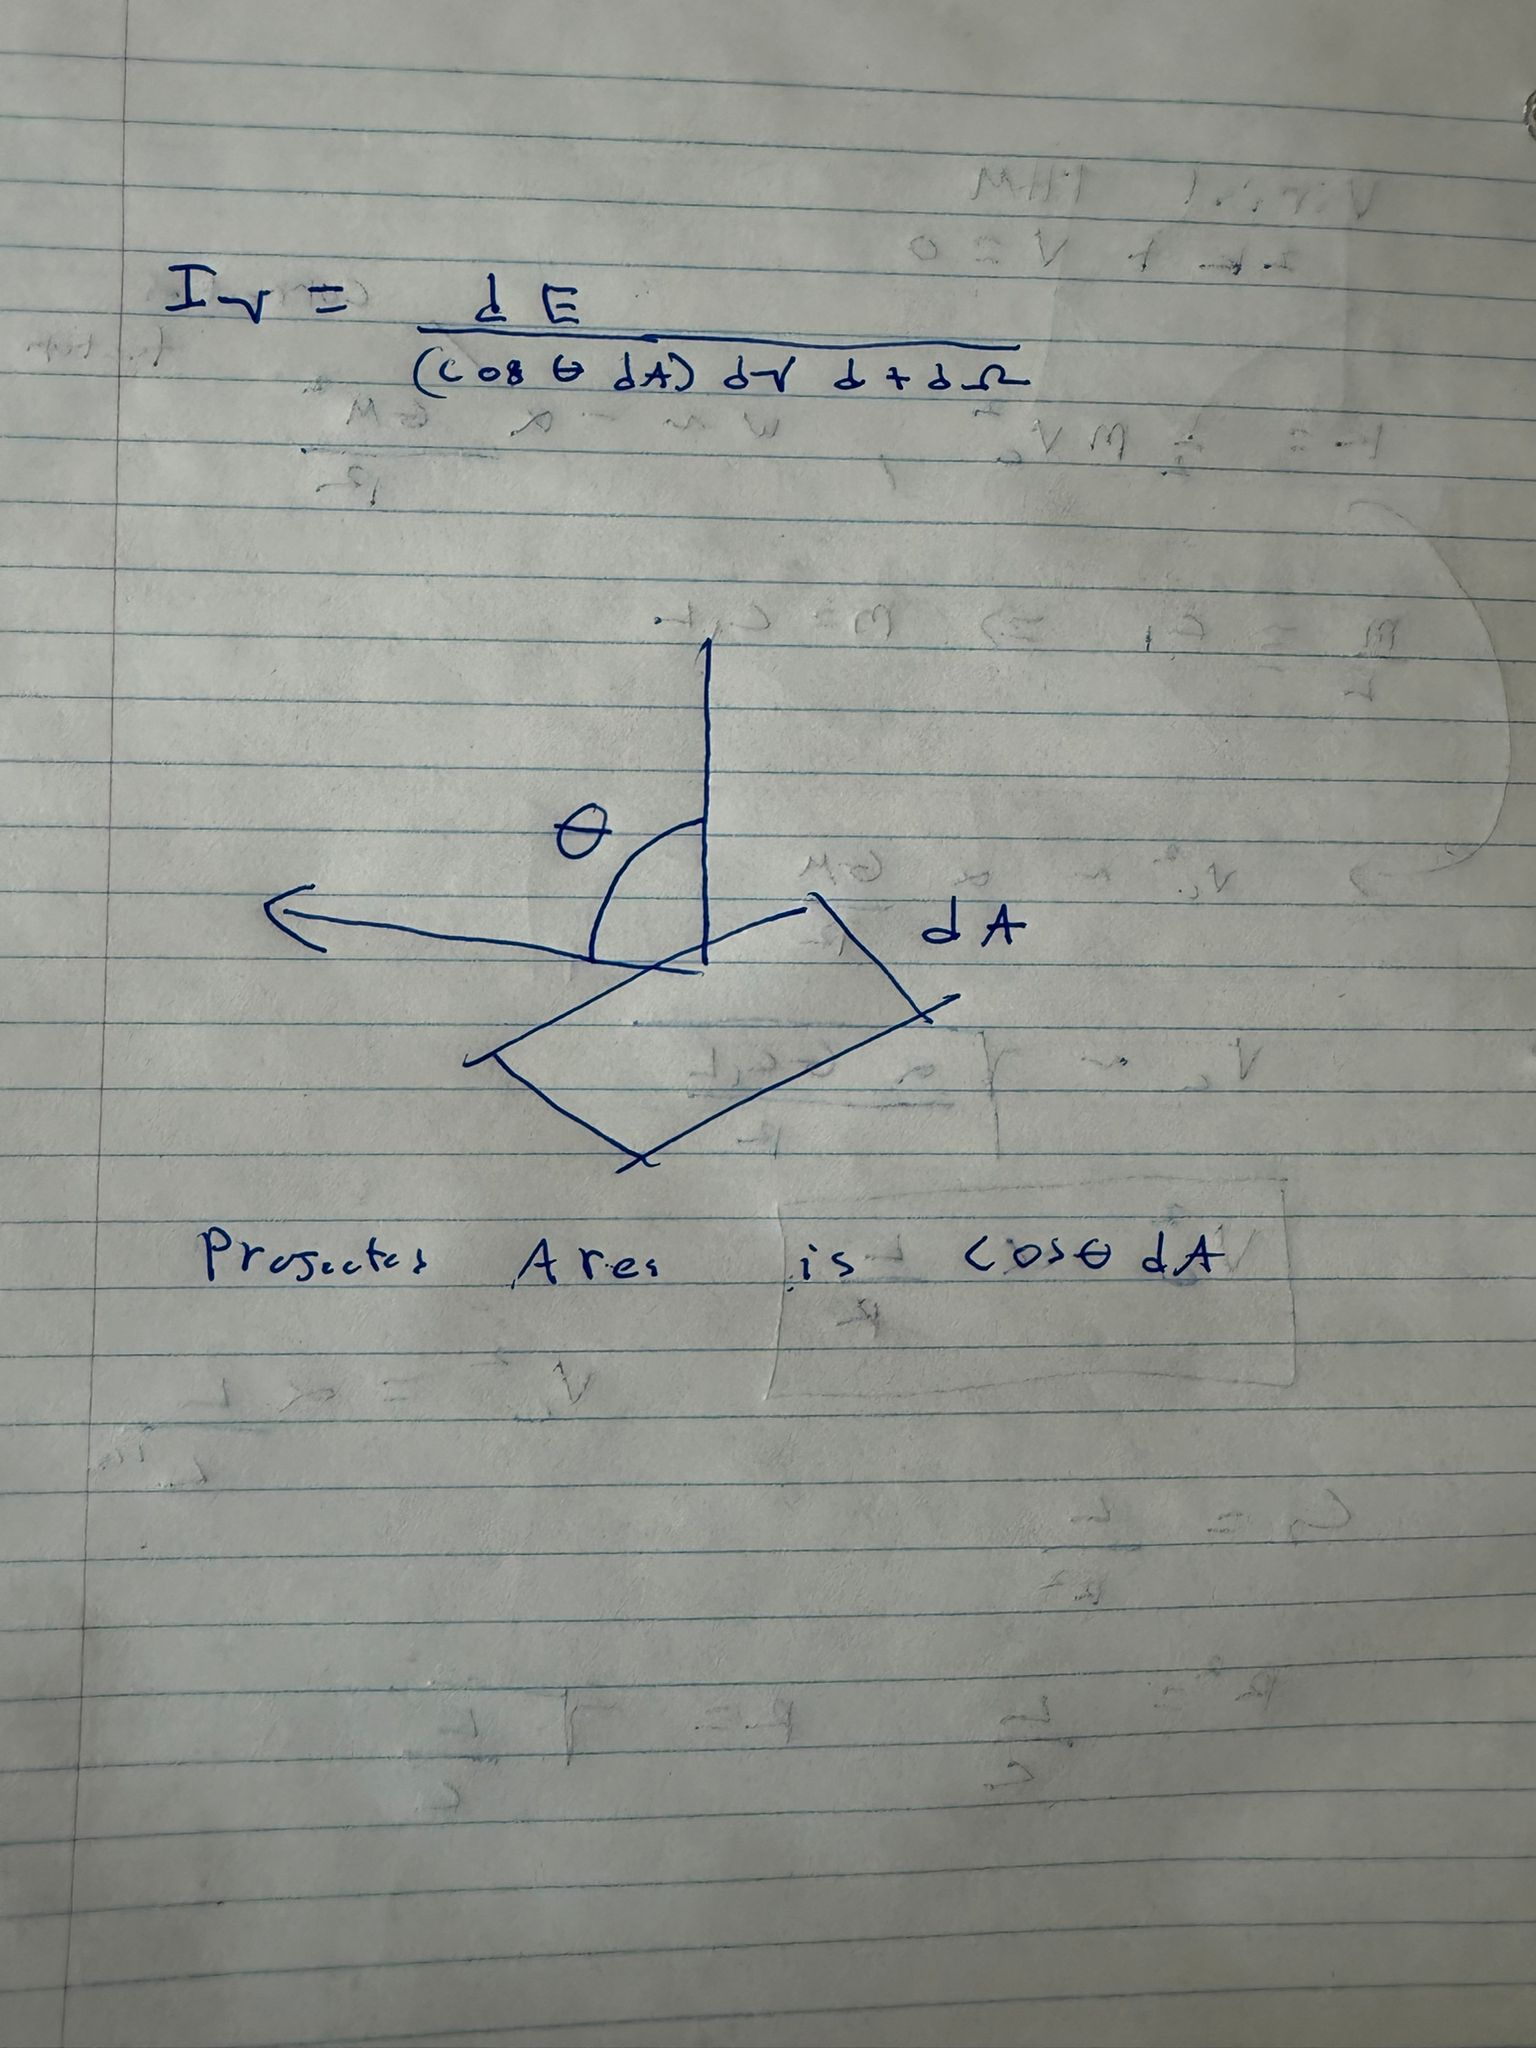
\includegraphics[width=0.75\linewidth]{images/problem_3_diagram.jpeg}
    \caption{Geometry of specific intensity.}
    \label{fig:probem_3_diagram}
\end{figure}

Where $ I_\nu$ is the specific intensity, $dE$ is energy emitted, $\cos\theta dA$ is the projected 2D area (see Figure \ref{fig:probem_3_diagram}for geometry), $dt$ is the per time, and $d\nu$ is per frequency, and $d\Omega$ is our solid angle. 



Let's have two people ( or the sun and a small solar panel if you will), the question is if they agree on the specific intensity:
\begin{equation}
    I_\nu \stackrel{?}{=} I_{\nu}^{'}
\end{equation}

\begin{equation}
    \frac{dE}{(\cos\theta dA)dtd\nu d\Omega} \stackrel{?}{=} \frac{dE^{'}}{(\cos\theta^{'} dA^{'})dt^{'}d\nu^{'} d\Omega^{'}}
\end{equation}

Due to symmetry, the solid angle, and $\theta$'s cancel Assuming classical physics, $dt$, and $d\nu$ are also the same for both people\footnote{$d\Omega = \frac{cos\theta^{'}da^{'}}{r^2}$, and  $d\Omega^{'} = \frac{cos\theta^{}da^{}}{r^2}$, where $r$ is the distance between the two people.}. 

\begin{equation}
    \boxed{dE = dE^{'}}
\end{equation}
therefor, specific intensity is conserved (does not vary with distance). 